\ylDisplay{Antikaitse} % Ülesande nimi
{Kaur Aare Saar} % Autor
{piirkonnavoor} % Voor
{2020} % Aasta
{P 9} % Ülesande nr.
{2} % Raskustase
{
% Teema: Elektriõpetus

\ifStatement
Antikaitse (joonisel $AK$) on seade, mis enne aktiveerumist käitub kui avatud lüliti (väga suure takistusega takisti). Kui aga antikaitsele rakendada kõrge pinge, siis see aktiveerub, ning pärast seda käitub jäädavalt kui suletud lüliti. Antikaitsmeid kasutatakse näiteks jadamisi ühendatud jõuluküünaldes, et tagada pärast ühe lambi katkiminekut teiste lampide töötamine. Joonisel on elektriskeem, milles on kokku $n = 16$ jadamisi ühendatud ühesugust küünalt. Pinge skeemi otstel $V = 240$ $V$. Iga küünal on ühendatud rööpselt antikaitsega. Hetkel $t = 0$ küünal $A$ puruneb. Eeldada, et antikaitse aktiveerub, kui sellele on rakendunud pinge, mis on kõrgem kui $21$ $V$ kauemaks kui $\tau = 1$ $ms$, ja et iga küünal on ette nähtud töötama pingel kuni $24$ $V$. Kirjeldage, kuidas muutuvad pinged lampide klemmidel lambi $A$ katkimineku käigus.  Milline on minimaalne lampide arv, mis saavad korraga põleda?
\begin{center}
	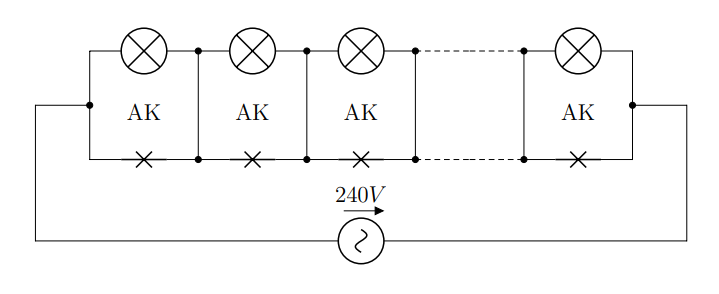
\includegraphics[width=0.5\linewidth]{2020-v2p-09-yl.png}
\end{center}
\fi

\ifHint
Igal ajahetkel peab kogu pingelangus olema $240$ V.
\fi


\ifSolution
Igal ajahetkel peab kogu pingelangus olema $240$ V. Algul on see jaotunud kõikide lampide vahel võrdselt, seega igal on lambil pingelangus $\frac{240 V}{16} = 15$ V. Vahemikus $0$ kuni $\tau$ ei liigu läbi ühegi lambi voolu. Seega pingelangus tervetel lampidel on $0$ V. Kuna summaarselt peab pingelangus olema kõikidel lampidel kokku $240$ V, siis on lambil $A$ pingelangus $240$ V. Alates hetkest $\tau$ käitub lambiga $A$ rööpselt ühendatud antikaitse kui suletud lüliti, seega seal pingelangus puudub ja lambil olev pingelangus on $0$ V. Pingelangus teiste lampide vahel jaotub võrdselt, seega kõikidel teistel lampidel on pingelangus $\frac{240 V}{15} = 16$ V. Kui lambil olev pinge tõuseb üle $21$ V, siis antikaitse aktiveerub. Järelikult lampide arv, mis saab korraga põleda peab olema suurem kui $\frac{240 V}{21 V} = 11,4$. Seega korraga saab põleda minimaalselt $12$ lampi. Kui terveks on jäänud vaid $11$ lampi, siis oleks igal lambil pingelangus $\frac{240 V}{11}= 21,8$ V, mis aktiveeriks kõik antikaitsmed, mis lühistaks pingeallika.
\fi
}